
\documentclass{article}

\usepackage{amssymb}
\usepackage{amsmath}
\usepackage{pgfplots}
\usepackage{tikz}
\usepackage[top=0.9in, bottom=0.9in, left=1.5in, right=1.5in]{geometry}
\usepackage{xcolor}
\usepackage{xparse,mathtools}


\title{ECE421 Problem Set 3}
\author{Micol Altomare}
\date{October 11, 2023} 

\pgfplotsset{compat=1.17}
\DeclareMathOperator*{\minimize}{min}


\begin{document}

\maketitle


\section{SVM with Hard Margin}



\subsection{}
By inspection, the equation of the maximum-margin hyperplane is $\boxed{x_2=-x_1+1.5}$. %%%% CHECK format!!!! (refer to video notes)


\begin{figure}[ht]
  \centering
  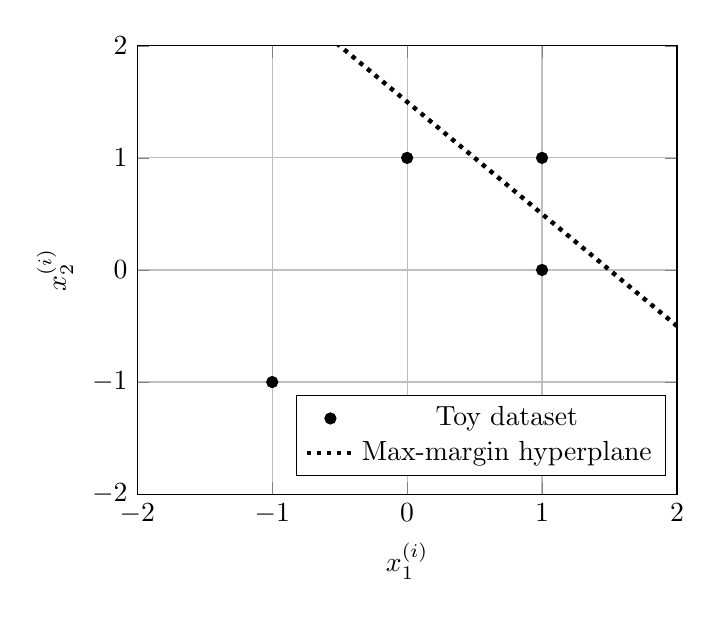
\begin{tikzpicture}
    \begin{axis}[
      xlabel={$x_1^{(i)}$},
      ylabel={$x_2^{(i)}$},
      xmin=-2, xmax=2, 
      ymin=-2, ymax=2,
      xtick={-2,-1,0,1,2},
      ytick={-2,-1,0,1,2},
      grid=both,
      legend style={at={(0.98,0.04)},anchor=south east}
      ]
      
     \addplot[only marks, mark=*] coordinates {
        (1, 1) % x1 (Red)
        (-1, -1) % x2 (Blue)
        (1, 0) % x3 (Blue)
        (0, 1) % x4 (Blue)
      };
      \addlegendentry{Toy dataset}
      \addplot [dotted, domain=-2:2, samples=2, ultra thick] {-1*x + 1.5};
      \addlegendentry{Max-margin hyperplane} 
    \end{axis}
  \end{tikzpicture}
  \caption{Scatter plot of the toy dataset.}
\end{figure}

% TODO: labelling + caption
% TODO: ensure correc form for the hyperplane equation



\subsection{}
$\boxed{x^{(1)}, x^{(3)}, x^{(4)}}$ are support vectors since they are closest to the hyperplane, and since their margin constraint will be 1 (ie. they are on the margin).
% TODO: double check reasoning

\subsection{}
Recall the Lagrange function: $$ L (\bar{x}, \lambda) = f_0 (\bar{x}) + \sum_{i=1} \lambda_i f_i (\bar{x}), \lambda_i \geq 0 $$
Given optimization problem:
\begin{align*}
 \displaystyle{\minimize_{\vec{w}, b}} & \; \frac{1}{2} || \vec{w}||^2 \; \text{s.t.} \; (\vec{w} \cdot \vec{x}^{(j)} + b)y^{(j)} \geq 1 \; \forall j \\
\text{Objective function:} \; & f_0(\bar{x}) = \frac{1}{2} || \vec{w} || ^2 \\
\text{Constraint:} \; & (\vec{w} \cdot \vec{x}^{(j)} + b)y^{(j)} \geq 1 \forall j \\
\implies & (\vec{w} \cdot \vec{x}^{(j)} + b)y^{(j)} -1 \geq 0 \forall j \\
\implies &\boxed{	L(\vec{w}, b, \vec{\alpha}) = \frac{1}{2} || \vec{w} || ^2 - \sum_j \alpha_j [ (\vec{w} \cdot \vec{x}^{(j)} + b)y^{(j)} -1]}
\end{align*}



\subsection{}
$$ \displaystyle{\minimize_{\vec{w}, b}} L(\vec{w}, b, \vec{\alpha}) \implies \frac{\partial}{\partial \vec{w}} L(\vec{w}, b, \vec{\alpha}) = 0,  \frac{\partial }{\partial b} L(\vec{w}, b, \vec{\alpha}) = 0 $$
Given the result from \textbf{1.3}, \\
\begin{align*}
 \frac{\partial}{\partial \vec{w}} L(\vec{w}, b, \vec{\alpha}) &= \vec{w} - \sum_j \alpha_j y^{(j)} \vec{x}^{(j)} = 0 \\
 \implies & \boxed{\vec{w} =  \sum_j \alpha_j y^{(j)} \vec{x}^{(j)}} \\
  \frac{\partial}{\partial b} L(\vec{w}, b, \vec{\alpha}) &= - \sum_j \alpha_j y^{(j)} = 0 \\
  \implies & \boxed{0 = \sum_j \alpha_j y^{(j)}}
\end{align*}


\subsection{}
\begin{align*}
& \underset{\vec{\alpha}}{\text{max}}\;  \underset{\vec{w}, b}{\text{min}} L(\vec{w}, b, \vec{\alpha}) \\
=  & \;  \underset{\vec{\alpha}}{\text{max}}\;  \underset{\vec{w}, b}{\text{min}} \left(  \frac{1}{2} || \vec{w} || ^2 - \sum_j \alpha_j [ (\vec{w} \cdot \vec{x}^{(j)} + b)y^{(j)} -1] \right) \\
=  & \;  \underset{\vec{\alpha}}{\text{max}}\;  \left(  \frac{1}{2} || \vec{w} || ^2 - \sum_j (  \alpha_j \textcolor{blue}{\vec{w}} \cdot \vec{x}^{(j)} y^{(j)} + \textcolor{red}{\alpha_j b y^{(j)}} -\alpha_j ) \right) \\
\text{Given the results from \textbf{1.4},} \\
= & \;  \underset{\vec{\alpha}}{\text{max}}\;  \left( \frac{1}{2} \textcolor{orange}{|| \vec{w} || ^2} - \sum_j \alpha_j \vec{x}^{(j)} y^{(j)} \textcolor{blue}{\sum_k \alpha_k y^{(k)} \vec{x}^{(k)}} + \sum_j \alpha_j \right) \\
= & \;  \underset{\vec{\alpha}}{\text{max}}\; \left(\frac{1}{2} \textcolor{orange}{\sum_j \sum_k \alpha_j \alpha_k y^{(j)} y^{(k)} (\vec{x}^{(j)} \cdot \vec{x}^{(k)} )} - \sum_j \sum_k \alpha_j \alpha_k y^{(j)} y^{(k)} (\vec{x}^{(j)} \cdot \vec{x}^{(k)} ) + \sum_j \alpha_j \right) \\
& = \boxed{\underset{\vec{\alpha}}{\text{max}}\; \left( \sum_j \alpha_j - \frac{1}{2} \sum_j \sum_k \alpha_j \alpha_k y^{(j)} y^{(k)} (\vec{x}^{(j)} \cdot \vec{x}^{(k)} ) \right)}
\end{align*}

\subsection{}
Original constraint: $$ (\vec{w} \cdot \vec{x}^{(j)} + b) y^{(j)} \geq 1 \; \forall j$$
From \textbf{1.1}, $\vec{x}^{(2)} $ is the only non-support vector. From the Lagrange function, if the original constraint does not apply for non-support vectors, then $ \sum_j \alpha_j (\vec{w} \cdot \vec{x}^{(j)} + b) y^{(j)} - 1 $ must be zero. Thus, $\alpha_j$ corresponding to the non-support vector must be zero. $\boxed{\therefore \alpha_{j*} = 0 \; \text{when} \; j^* = 2}$.

\subsection{}
Using the second result from \textbf{1.4} and the dataset,
\begin{align*}
0 &= \sum_{j=1}^4 \alpha_j y^{(j)} \\
&= \alpha_1 y^{(1)} + \alpha_2 y^{(2)} + \alpha_3 y^{(3)} + \alpha_4 y^{(4)} \\
&= \alpha_1 (1) + 0(-1) + \alpha_3 (-1) + \alpha_4 (-1) \\
&= \alpha_1 - \alpha3 - \alpha_4 \\
\implies & \boxed{\alpha_1 = \alpha_3 + \alpha_4}
\end{align*}



\subsection{}
To solve the optimization problem from \textbf{1.5}, we can expand the optimization problem and utilize the dataset points, positive/negative class assignments and the deduced dual value relationships: $\alpha_2 = 0, \alpha_1 = \alpha_3 + \alpha_4 \implies \alpha_3 = \alpha_1 - \alpha_4, \alpha_4 = \alpha_1 - \alpha_3$.  

\begin{align*}
& \underset{\vec{\alpha}}{\text{max}}\; \left( \sum_{j=1}^4 \alpha_j - \frac{1}{2} \sum_{j=1}^4 \sum_{k=1}^4 \alpha_j \alpha_k y^{(j)} y^{(k)} (\vec{x}^{(j)} \cdot \vec{x}^{(k)} ) \right) \\
= \; & \underset{\vec{\alpha}}{\text{max}}\; \left( \alpha_1 + \alpha_3 + \alpha_4 - \frac{1}{2} \sum_{j=1}^4  \alpha_j   y^{(j)} \sum_{k=1}^4 \alpha_k y^{(k)} (\vec{x}^{(j)} \cdot \vec{x}^{(k)} ) \right) \\
= \; & \underset{\vec{\alpha}}{\text{max}}\; \left( \alpha_1 + \alpha_3 + \alpha_4 - \frac{1}{2} \left( \alpha_1(2\alpha_1 - \alpha_3 - \alpha_4) + 0 - \alpha_3 (\alpha_1 - \alpha_3) - \alpha_4 (\alpha_1 - \alpha_4     ) \right) \right) \\
= \; & \underset{\vec{\alpha}}{\text{max}}\; \left( 2 \alpha_3 + 2 \alpha_4 - \frac{1}{2} \left( 2\alpha_1^2 - \alpha_1 \alpha_3  - \alpha_1 \alpha_4 - \alpha_3 \alpha_1 + \alpha_3^2 - \alpha_4 \alpha_1 + \alpha_4^2     \right) \right) \\
= \; & \underset{\vec{\alpha}}{\text{max}}\; \left( 2 \alpha_3 + 2 \alpha_4 - \frac{1}{2} \left( \textcolor{brown}{2\alpha_1^2 - 2 \alpha_1 \alpha_3  -2 \alpha_1 \alpha_4} + \alpha_3^2  + \alpha_4^2     \right) \right) \\
= \; & \underset{\vec{\alpha}}{\text{max}}\; \left( 2 \alpha_3 + 2 \alpha_4 - \frac{1}{2} \left( \alpha_3^2  + \alpha_4^2     \right) \right) \\
\text{Note:} \; & \textcolor{brown}{2\alpha_1^2 - 2\alpha_1 \alpha_3 - 2\alpha_1 \alpha_4} = 
2 \alpha_1^2 - 2\alpha_1 (\alpha_1 - \alpha_4) - 2 \alpha_1 (\alpha_1 - \alpha_3) = 
2\alpha_1^2 - 2\alpha_1^2 + 2\alpha_1(\alpha_3 + \alpha_4) - 2\alpha_1^2 = 0 
\end{align*}
Now, we may take the partial derivatives of the simplified optimization problem and set them to zero:
\begin{align*}
\frac{\partial}{\partial \alpha_3} \left( 2 \alpha_3 + 2 \alpha_4 - \frac{1}{2} \left( \alpha_3^2  + \alpha_4^2     \right) \right) &= 2-\alpha_3 = 0 \\ \implies \alpha_3 &= 2 \\
\frac{\partial}{\partial \alpha_4} \left( 2 \alpha_3 + 2 \alpha_4 - \frac{1}{2} \left( \alpha_3^2  + \alpha_4^2     \right) \right) &= 2-\alpha_4 = 0 \\ \implies \alpha_4 &= 2 \\
\alpha_1 &= \alpha_3 + \alpha_4 \\
\implies \alpha_1 &= 4 \\
\boxed{\therefore \vec{\alpha} = \begin{bmatrix} \alpha_1 \\ \alpha_2 \\ \alpha_3 \\ \alpha_4 \end{bmatrix} = \begin{bmatrix} 4 \\ 0 \\ 2 \\ 2 \end{bmatrix}		}
\end{align*}




























\subsection{}
Using the first result from \textbf{1.4}, \textbf{1.8}, and the dataset,
\begin{align*}
\vec{w} &= \sum_j \alpha_j y^{(j)} \vec{x}^{(j)} \\
&= \alpha_1 y^{(1)} \vec{x}^{(1)} + \alpha_2 y^{(2)} \vec{x}^{(2)} + \alpha_3 y^{(3)} \vec{x}^{(3)} + \alpha_4 y^{(4)} \vec{x}^{(4)} \\
&= 4 \begin{bmatrix} 1 \\ 1 \end{bmatrix} - 2 \begin{bmatrix} 1 \\ 0 \end{bmatrix} - 2 \begin{bmatrix} 0 \\ 1 \end{bmatrix} \\
&= \begin{bmatrix} 4-2-0\\ 4-0-2 \end{bmatrix} \\
& \boxed{\vec{w} = \begin{bmatrix} 2 \\ 2 \end{bmatrix}}
\end{align*}

\subsection{}
Original constraint: $$ (\vec{w} \cdot \vec{x}^{(j)} + b) y^{(j)} \geq 1 \; \forall j$$
For support vectors, the constraint is tight: $$ (\vec{w} \cdot \vec{x}^{(j)} + b) y^{(j)} = 1 \; \forall j$$
Any of the support vectors can be used to determine $b$, like $x^{(1)}$:
\begin{align*}
(\vec{w} \cdot \vec{x}^{(1)} + b) y^{(1)} = 1 \\
\left( \begin{bmatrix} 2 \\ 2 \end{bmatrix} \cdot \begin{bmatrix} 1 \\ 1 \end{bmatrix} + b \right) 1 = 1 \\
4 + b = 1 \\
\implies \boxed{b = -3 }
\end{align*}











\end{document}
